\section{Lévi Function N.13}
\label{sec:app:test:levi}
  The \emph{Lévi function N.13} is a noteworthy two-dimensional function 
  frequently employed in the field of optimization algorithms for performance 
  testing. 
  Its complex, sinuous landscape, teeming with numerous local minima, presents a 
  significant challenge to optimization procedures.

  \begin{definition}[Lévi Function N.13]
    \label{def:app:test:levi}
    The \emph{Lévi function N.13}, denoted as \(f: \mathbb{R}^2 \rightarrow 
    \mathbb{R}\), is formally defined as follows:

    \begin{equation}
      \label{eq:app:test:levi}
      f(x,\, y) = \sin^2(3\pi x) 
        + (x - 1)^2 \cdot (1 + \sin^2(3\pi y)) 
        + (y - 1)^2 \cdot (1 + \sin^2(2\pi y))
    \end{equation}
    
    where \(x,\, y \in \mathbb{R}\) are the decision variables.
  \end{definition}

  The Lévi function N.13 finds its global minimum at \(f(1, 1) = 0\). 
  The complex topology of this function is visually captured in the contour and 
  surface plots shown in Figure \ref{fig:app:test:levi}.

  \begin{figure}[ht!]
    \centering
    \begin{subfigure}[b]{0.45\textwidth}
      \centering
      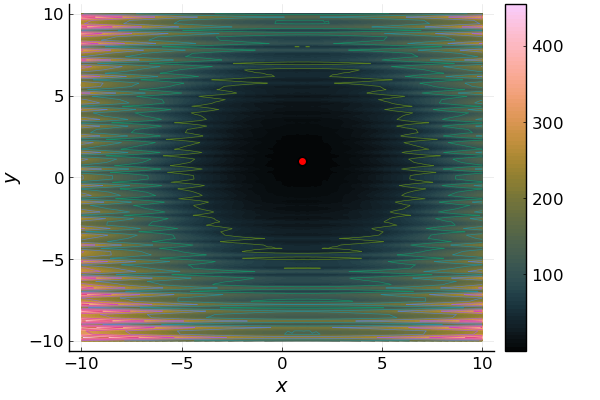
\includegraphics[width=\textwidth]{img/test_functions/levi_contour.png}
      \caption{Contour plot of the Lévi function N.13}
      \label{fig:app:test:levi:contour}
    \end{subfigure}
    \hfill
    \begin{subfigure}[b]{0.45\textwidth}
      \centering
      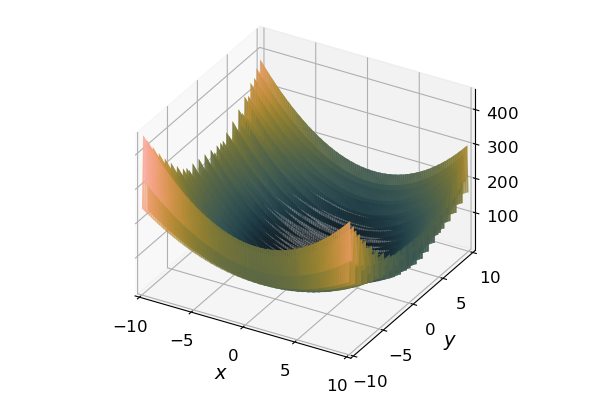
\includegraphics[width=\textwidth]{img/test_functions/levi_surface.png}
      \caption{Surface plot of the Lévi function N.13}
      \label{fig:app:test:levi:surface}
    \end{subfigure}
    \caption{Contour and Surface Representations of the Lévi Function N.13}
    \label{fig:app:test:levi}
  \end{figure}
